\chapter{Diodes}

\section{Semiconductors}

\subsection{Intrinsic Semiconductor}

An intrinsic semiconductor, also called as undoped semiconductor, is a pure semiconductor without and significant dopant species present. Two factors are responsible to the current pass through it:

\begin{itemize}
\item Excited electrons
\item Holes
\end{itemize}

However, we seldom use intrinsic semiconductors.

\subsection{Extrinsic Semiconductor}

An extrinsic semiconductor is a semiconductor that has been doped, which has more features and provides more charge carriers.

\subsubsection{P-type semiconductor}

P-type semiconductors are created by doping some electron accepter elements during manufacture. It has more holes, holes are major carriers of the current.

\subsubsection{N-type semiconductor}

N-type semiconductors are created by doping some electron donor elements during manufacture. It has more electrons, electrons are major carriers of the current.

\section{P-N Junction and Diode}

When we combine the 2 types of extrinsic semiconductor together, we found some interesting features. As p-type semiconductors use holes to transmit currents, n-type semiconductors use electrons to transmit currents, and, to make life easier, we take holes as positive charges. When the two types of semiconductors are put together, at the contact surface, diffusion phenomenon occur.

Some holes traveled into the n-type semiconductor, some electrons traveled into the p-type semiconductor. And after that, an inner electric field formed, which hinders the p-n junction from carrying currents.

To ease the effect above, we need to add some positive voltage at p-type semiconductor, and also add some negative voltage at n-type semiconductor. And if we add negative voltage at n-type semiconductor, positive voltage at p-type semiconductor, the effect will be intensified.

\begin{figure}[H]
  \centering
  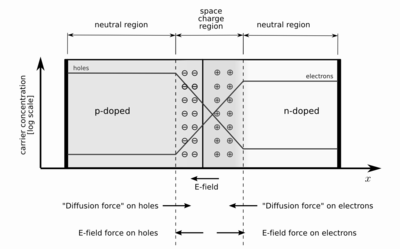
\includegraphics[width=0.5\linewidth]{figures/Pn-junction-equilibrium.png}
  \caption{PN Junction at equilibrium state}
  \label{fig:}
\end{figure}

In conclusion, if we add forward voltage (from p to n), the diode acts as a short circuit. If we add reversed voltage, the diode acts like an open circuit. And if the reversed voltage is big enough, it will cause the diode broken-through, and the current flow through it will increase tremendously.

\subsection{Breakdown of P-N Junction}

There are two types of breakdown

\begin{itemize}
\item electricity breakdown, which is invertible
\item heat breakdown, which cause permanent damage
\end{itemize}

\section{Diode modeling}

\subsection{Mathematically idealized diode}

Firstly, consider a mathematically idealized diode. In such an ideal diode, if the diode is reverse biased, the current flowing through it is zero. This ideal diode starts conducting at 0 V and for any positive voltage an infinite current flows and the diode acts like a short circuit. The I-V characteristics of an ideal diode are shown below:

\begin{figure}[H]
  \centering
  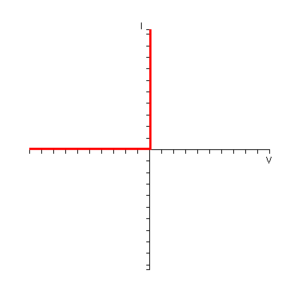
\includegraphics[width=0.4\linewidth]{figures/Diode_Modelling_Image5.png}
  \label{fig:}
  \caption{I-V characteristic of an ideal diode.}
\end{figure}

\subsection{Ideal diode in series with voltage source}

Now consider the case when we add a voltage source in series with the diode in the form shown below:

When forward biased, the ideal diode is simply a short circuit and when reverse biased, an open circuit.

\begin{figure}[H]
  \centering
  \begin{subfigure}{.4\textwidth}
    \centering
    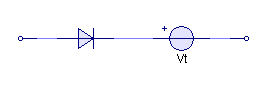
\includegraphics[width=\linewidth]{figures/Diode_Modelling_Image6}
    \caption{Ideal diode with a series voltage source.}
    \label{fig:}
  \end{subfigure}%
  \begin{subfigure}{.4\textwidth}
    \centering
    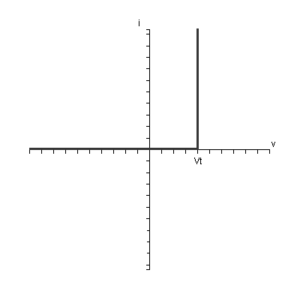
\includegraphics[width=\linewidth]{figures/Diode_Modelling_Image8}
    \caption{I-V characteristic of an ideal diode with a series voltage source.}
    \label{fig:}
  \end{subfigure}
  \caption{Ideal diode in series with voltage source}
  \label{fig:}
\end{figure}

\subsection{Diode with voltage source and current-limiting resistor}

The last thing needed is a resistor to limit the current, as shown below:

\begin{figure}[H]
  \centering
  \begin{subfigure}{.4\textwidth}
    \centering
    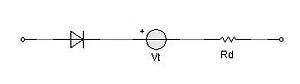
\includegraphics[width=\linewidth]{figures/Diode_Modelling_Image9}
    \caption{Ideal diode with a series voltage source and resistor.}
    \label{fig:}
  \end{subfigure}%
  \begin{subfigure}{.4\textwidth}
    \centering
    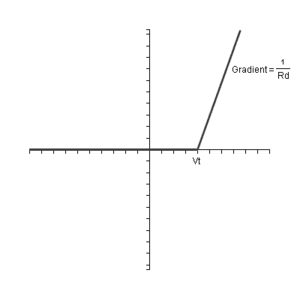
\includegraphics[width=\linewidth]{figures/Diode_Modelling_Image11}
    \caption{I-V characteristic of an ideal diode with a series voltage source and resistor.}
    \label{fig:}
  \end{subfigure}
  \caption{Diode with voltage source and current-limiting resistor}
  \label{fig:}
\end{figure}

The real diode now can be replaced with the combined ideal diode, voltage source and resistor and the circuit then is modelled using just linear elements. If the sloped-line segment is tangent to the real diode curve at the Q-point, this approximate circuit has the same small-signal circuit at the Q-point as the real diode.

\subsection{Diode in Small Signal Circuits}

\begin{figure}[H]
  \centering
  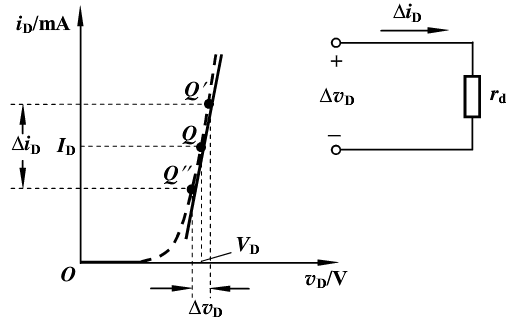
\includegraphics[width=0.5\linewidth]{figures/Diode-Small-Signal}
  \caption{I-V Characteristic of Diode in Small Signal}
  \label{fig:}
\end{figure}

\begin{equation*}
  \begin{aligned}
    r_d = \dfrac{1}{g_d} = \dfrac{V_T}{I_{DQ}}  
  \end{aligned}
\end{equation*}

Where, in the condition of $T = 300 \  \mathrm{K}$,

\begin{equation*}
  \begin{aligned}
    V_T = 26 \  \mathrm{mV}
  \end{aligned}
\end{equation*}

\section{Applications of Diodes}

\subsection{Rectifier Circuit}

\begin{figure}[H]
  \centering
  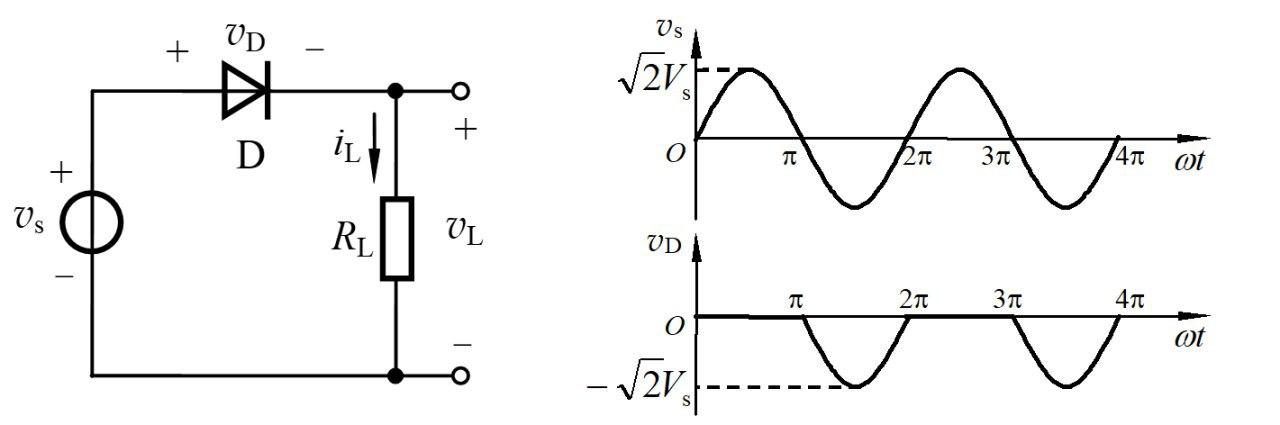
\includegraphics[width=0.5\linewidth]{figures/RectifierCircuit}
  \caption{A Simple Rectifier Circuit}
  \label{fig:}
\end{figure}
\begin{figure}[H]
  \centering
  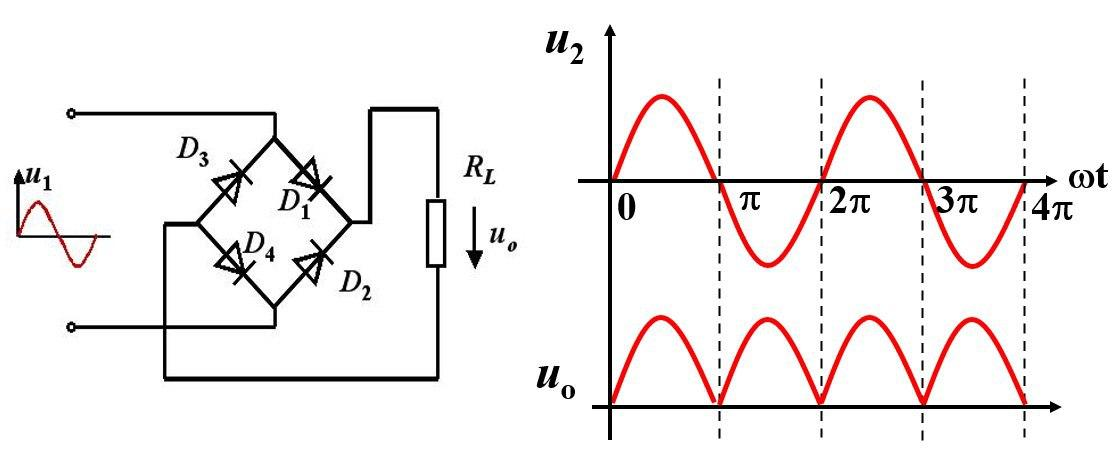
\includegraphics[width=0.5\linewidth]{figures/BridgedRectifierCircuit}
  \caption{A Bridged Rectifier Circuit}
  \label{fig:}
\end{figure}

\subsection{Limiting Circuit}

\begin{figure}[H]
  \centering
  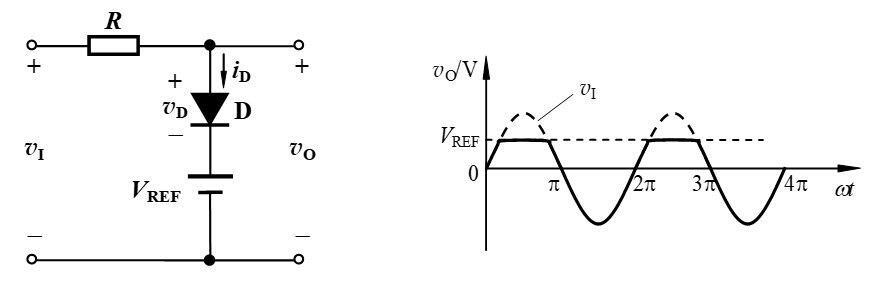
\includegraphics[width=0.5\linewidth]{figures/LimitingCircuit}
  \caption{A Limiting Circuit}
  \label{fig:}
\end{figure}

\subsection{Switching Circuit}

\begin{figure}[H]
  \centering
  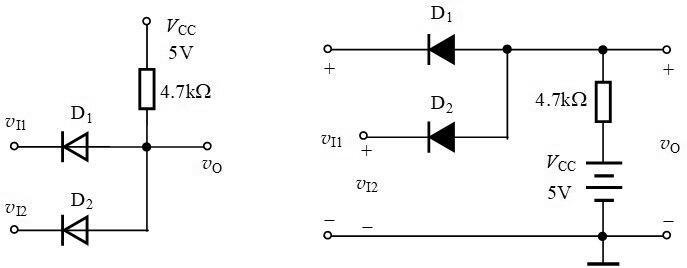
\includegraphics[width=0.5\linewidth]{figures/SwitchCircuit}
  \caption{A Switching Circuit, $v_o = 5 \  \mathrm{V}$ holds only if all the input voltage is $5 \  \mathrm{V}$}
  \label{fig:}
\end{figure}

\section{Diodes for Special Usage}

\subsection{Zener diode}

A Zener diode is manufactured to be broken-through. It is used to stabilize voltages. As we can know from the I-V characteristic of an diode, when the diode is broken-through, change in current only cause little change in voltage.

\begin{figure}[H]
  \centering
  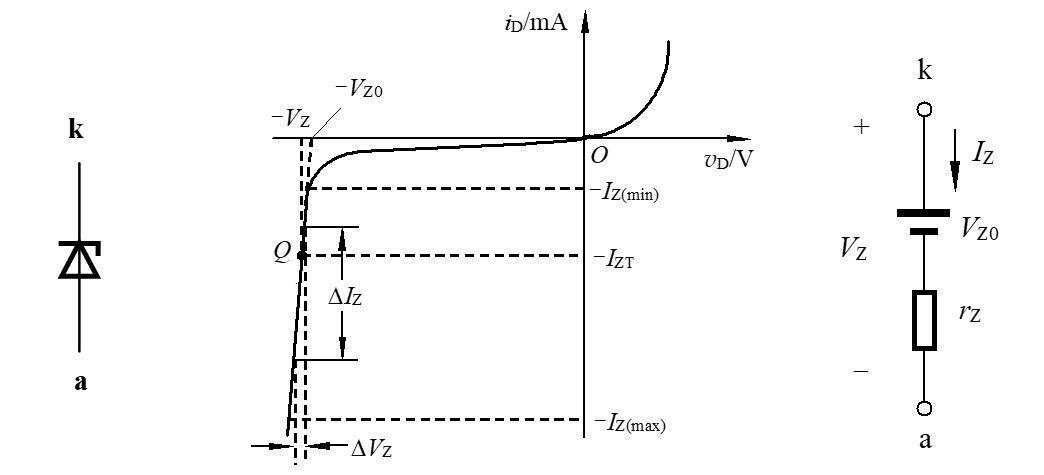
\includegraphics[width=0.5\linewidth]{figures/Zener-diode-1}
  \caption{Zener Diode's electronic symbol and I-V characteristic}
  \label{fig:}
\end{figure}

\subsection{Photodiode}

A photodiode is a semiconductor device that converts light into an electrical current. The current is generated when photons are absorbed in the photodiode.

\subsection{Light-emitting diode}

A light-emitting diode (LED) is a semiconductor light source that emits light when current flows through it.

\subsection{Schottky diode}

The Schottky diode (named after the German physicist Walter H. Schottky), also known as Schottky barrier diode or hot-carrier diode, is a semiconductor diode formed by the junction of a semiconductor with a metal. It has a low forward voltage drop and a very fast switching action.



%%% Local Variables:
%%% mode: latex
%%% TeX-master: "Analogue_Electronics"
%%% End:
